\documentclass[a4paper, fleqn]{report}

\usepackage[T2A]{fontenc}
\usepackage[utf8]{inputenc}
\usepackage[russian]{babel}

\usepackage{amsmath}
\usepackage{geometry}
\usepackage{graphicx}
\usepackage{hyperref}
\usepackage{enumitem}
\usepackage{listings}
\usepackage{titlesec}
\usepackage{tocbibind}
\usepackage{xcolor}

\geometry{top=2cm, bottom=2cm, left=2.5cm, right=2.5cm}

\hypersetup{
    colorlinks=true,
    linkcolor=blue,
    urlcolor=blue
}

\titleformat{\chapter}[block]
{\normalfont\huge\bfseries}{}{0em}{}

\lstset{
    basicstyle=\ttfamily\footnotesize,
    keywordstyle=\bfseries\color{blue},
    commentstyle=\itshape\color{gray},
    stringstyle=\color{red},
    numbers=left,
    numberstyle=\small,
    stepnumber=1,
    breaklines=true,
    frame=single,
    tabsize=4,
    captionpos=b,
}

\title{
\textbf{Московский Государственный Университет имени М.В.\ Ломоносова}\\
\textbf{Факультет вычислительной математики и кибернетики}\\
\textbf{Введение в численные методы}\\
Отчёт по практическому заданию
}

\author{
Студент Кибизов Кирилл, группа 207
}
\date{\number\year}

\begin{document}

\maketitle

\tableofcontents

\chapter{Постановка задачи}

\section*{Дано:}
\begin{enumerate}[label=\arabic*.]
\item Уравнение в частных производных с граничными условиями:
\[
\begin{cases}
k_x \frac{\partial^2 u}{\partial x^2} + k_y \frac{\partial^2 u}{\partial y^2} = 0, \quad (x, y) \in [0, 1] \times [0, 1], \\
u(x, 0) = 0, \quad x \in [0, 1] \\
u(0, y) = 0, \quad y \in [0, 1] \\
u(x, 1) = \sin(\pi x), \quad x \in [0, 1] \\
u(1, y) = 0, \quad y \in [0, 1] \\
\end{cases}
\]
\item Разностная схема:
\[
\begin{cases}
k_x \dfrac{u_{i+1,j} - 2u_{i,j} + u_{i-1,j}}{h^2} + k_y \dfrac{u_{i,j+1} - 2u_{i,j} + u_{i,j-1}}{h^2} = 0, \quad i = \overline{1,N-1},\ j = \overline{1,N-1}, \\
u_{i,0} = 0, \quad i = \overline{0,N}, \\
u_{0,j} = 0, \quad j = \overline{0,N}, \\
u_{i,N} = 0, \quad i = \overline{0,N}, \\
u_{N,j} = 0, \quad j = \overline{0,N}.
\end{cases}
\]
где
\[
u_{i,j} \approx u(x_i, y_j), \quad x_i = \dfrac{i}{N}, \quad y_j = \dfrac{j}{N}, \quad h = \dfrac{1}{N}.
\]
\item Аналитическое решение данной задачи:
\[
u(x, y) = \dfrac{\sinh(\pi y / \sqrt{k_y})}{\sinh(\pi / \sqrt{k_y}))} \sin(\pi x)
\]
\end{enumerate}

\section*{Задача:}
\textbf{Требуется решить данную СЛАУ с помощью итерационного метода Якоби (где он применим)} для $N = 100$, рассматривая следующие случаи:
\begin{enumerate}
    \item $k_x = k_y = 1$,
    \item $k_x = 1$, $k_y = 10^6$.
\end{enumerate}
\textbf{В случае неприменимости итерационного метода Якоби предложить рабочий альтернативный метод.}


\chapter{Описание используемых числовых методов}

\subsection*{Итерационные алгоритмы}

При применении итерационных методов решения СЛАУ $Ax = f$ ответ получается в процессе построения последовательных приближений (итераций) $x_k = \{x_1^k, x_2^k, \dots, x_n^k\}$, сходящихся к решению исходной системы в пространстве $E_n$ с евклидовой нормой $\|x\|$: $\lim_{k \to \infty} x_k = x$, где $i$ - номер компоненты, а $k$ - номер итерации.

Сходимость обеспечивает принципиальную возможность получить в процессе итераций ответ с любой наперед заданной степенью точности. 

Если очередной член последовательности $x_{k+1}$ может выражаться только через предыдущий $x_{k+1} = F(x_k) $. Такие итерационные алгоритмы называют одношаговыми. Обычно линейно одношаговые алгоритмы записывают в стандартной канонической форме:
$B_{k+1} \frac{x_{k+1} - x_k}{\tau_{k+1}} + Ax_k = f$ и $\det B_{k+1} \neq$ и $\tau_{k+1} > 0$. В такой записи процесс характеризуется последовательностью матриц $B_{k+1}$ и числовых параметров $\tau_{k+1}$, которые называют итерационными параметрами.

\subsection*{Идея метода Якоби}
Метод Якоби строится на основе разностной схемы, в которой значения функции в каждом узле сетки обновляются независимо, используя значения с предыдущей итерации.

\subsection*{Идея метода верхней релаксации (SOR)}
Итерационная схема метода SOR
Метод SOR (Successive Over-Relaxation) представляет собой модификацию метода Зейделя, где значения в узлах обновляются последовательно и с учётом нового вычисленного значения, а также дополнительно корректируются с помощью параметра \(\omega\).

\chapter{Анализ применимости используемых числовых методов}

Перед тем как применять итерационные методы для решения системы линейных алгебраических уравнений (СЛАУ), необходимо убедиться, что они сходятся в рассматриваемом случае. Это включает в себя проверку структуры и свойств матрицы системы, а также оценку выполнения достаточных условий сходимости итерационных методов.

\section*{Достаточные условия сходимости итерационного процесса}

\subsection*{Самосопряжённость матрицы}
В одномерном случае в направлении $x$ вторая производная $\frac{\partial^2 u}{\partial x^2}$ аппроксимируется по формуле:
\[
\frac{\partial^2 u}{\partial x^2} \approx \frac{u_{i+1,j} - 2u_{i,j} + u_{i-1,j}}{h_x^2}.
\]
Важно, что коэффициенты при $u_{i+1,j}$ и $u_{i-1,j}$ одинаковы (оба равны $\frac{1}{h_x^2}$).  
Аналогично производится аппроксимация второй производной по оси $y$.
Благодаря симметрии разностной схемы все связи между узлами в матрице $A$ получаются парными и "зеркальными". Это говорит о симметричности матрицы. Известные значения на границах области не делают матрицу несимметричной, так как они просто выносятся в вектор правой части $f$. Таким образом, можно сделать вывод, что матрица $A$ — самосопряжённая. В случае вещественной матрицы (все элементы матрицы $A$ — вещественные) понятия самосопряжённости и симметричности совпадают.

\subsection*{Положительно определённая матрица}
Чтобы доказать, что матрица $A$ положительно определённая, нужно показать, что для любого ненулевого вектора $v$ выполняется неравенство: $v^T A v > 0$.
Рассмотрим выражение $v^T A v$. Это скаляр, который можно записать как:
\[
v^T A v = \sum_{i,j} v_{i,j} (Av)_{i,j}.
\]
Для матрицы $A$, полученной из разностной аппроксимации второго порядка, можно записать, что $A$ действует на вектор $v$ следующим образом:
\[
(Av)_{i,j} = \frac{k_x}{h^2}(v_{i+1,j} - 2v_{i,j} + v_{i-1,j}) + \frac{k_y}{h^2}(v_{i,j+1} - 2v_{i,j} + v_{i,j-1}).
\]
Подставим это в $v^T A v$ и раскроем сумму:
\[
v^T A v = \sum_{i,j} v_{i,j} \left( \frac{k_x}{h^2}(v_{i+1,j} - 2v_{i,j} + v_{i-1,j}) + \frac{k_y}{h^2}(v_{i,j+1} - 2v_{i,j} + v_{i,j-1}) \right).
\]
При раскрытии суммы оказывается, что многие члены сокращаются. Получаем:
\[
v^T A v = \sum_{i,j} \frac{k_x}{h^2} (v_{i+1,j} - v_{i,j})^2 + \frac{k_y}{h^2} (v_{i,j+1} - v_{i,j})^2.
\]
В выражении $v^T A v$ остались только суммы квадратов разностей значений $v$ в соседних узлах. Так как $k_x > 0$, $k_y > 0$ и $h > 0$, каждый член суммы неотрицателен. Так как $v^T A v$ является суммой строго неотрицательных слагаемых, и каждое из них положительно, если $v \neq 0$, то $v^T A v > 0$. Это доказывает, что матрица $A$ положительно определённая.

\subsection*{Теорема Самарского}
Пусть $A$ — самосопряжённая положительно определённая матрица:  
$A = A^T, \quad A > 0,$  
и $B = A - \frac{\tau}{2} A$ — положительно определённая матрица, $\tau$ — положительное число:  
$B = A - \frac{\tau}{2} A > 0.$

Можно утверждать, что для матрицы $A$, которая:
\begin{itemize}
    \item симметрична ($A^T = A$),
    \item положительно определённая ($v^T A v > 0$ для любого $v \neq 0$),
\end{itemize}
выполняются достаточные условия сходимости итерационных методов, таких как методы Якоби и верхней релаксации (SOR). 

\subsection*{Сходимость методов}
В итоге методы Якоби и верхней релаксации (SOR) применимы, к данной задаче, однако важно также учитывать:
\begin{itemize}
    \item \textbf{Точность решения:} Точность определяется выбранным критерием остановки (например, достижением малого значения невязки или изменения решения между итерациями).
    \item \textbf{Быстрота сходимости:} Для улучшения быстроты сходимости можно:
    \begin{itemize}
        \item уменьшить шаг $h$,
        \item использовать "ускоряющие" параметры, такие как $\omega$ в методе верхней релаксации,
    \end{itemize}
\end{itemize}
\newpage

\chapter{Результаты}
1ый столбец - координаты точек \\
2ой столбец - численное рещение \\
3ий столбец - аналитическое решение \\

\lstset{language=bash}
\begin{lstlisting}[title={Вывод метода Якоби дл 1го теста (для некоторых точек, покоординатно кратных 0.25)}]
./a.out
Please, input amount of tests (max 10): 1
Leave 3rd argument as 0 (for Jacobi) or as w (w = 1 for Gauss-Seidel; 1 < w < 2 for SOR)
Input kx and ky and w; for test #1: 1 1 0
...
u(0.250000, 0.500000) | 0.139489 | 0.140904
u(0.250000, 0.750000) | 0.319105 | 0.320099
u(0.250000, 1.000000) | 0.707107 | 0.707107
u(0.500000, 0.000000) | 0.000000 | 0.000000
...
u(0.500000, 0.750000) | 0.451283 | 0.452688
u(0.500000, 1.000000) | 1.000000 | 1.000000
u(0.750000, 0.000000) | 0.000000 | 0.000000
u(0.750000, 0.250000) | 0.052184 | 0.053187
...
--------
Test #1:
Iterations = 10247
\end{lstlisting}

\lstset{language=bash}
\begin{lstlisting}[title={Вывод метода SOR для 2го теста с w = 1.0 (для некоторых точек, покоординатно кратных 0.25)}]
guest@host:/media/sf_Shared/jacobi$ ./a.out
Please, input amount of tests (max 10): 1   
Leave 3rd argument as 0 (for Jacobi) or as w (w = 1 for Gauss-Seidel; 1 < w < 2 for SOR)
Input kx and ky and w; for test #1: 1 1000000 1.0
...
u(0.250000, 0.500000) | 0.140196 | 0.140904
u(0.250000, 0.750000) | 0.319612 | 0.320099
u(0.250000, 1.000000) | 0.707107 | 0.707107
u(0.500000, 0.000000) | 0.000000 | 0.000000
...
u(0.500000, 1.000000) | 1.000000 | 1.000000
u(0.750000, 0.000000) | 0.000000 | 0.000000
u(0.750000, 0.250000) | 0.052690 | 0.053187
u(0.750000, 0.500000) | 0.140214 | 0.140904
...
--------
Test #1:
Iterations = 5851
\end{lstlisting}
\newpage

\section*{Количество итераций до сходимости}
\begin{table}[h!]
    \centering
    \begin{tabular}{|c|c|c|}
        \hline
        \textbf{Случай} & \textbf{Метод Якоби} & \textbf{Метод Зейделя}\\
        \hline
        $k_x = k_y = 1$ & 10247 & 5851\\
        \hline
        $k_x = 1, k_y = 10^6$ & 13029 & 6553\\
        \hline
    \end{tabular}
    \caption{Количество итераций до сходимости для каждого метода}
\end{table}

\begin{table}[h!]
\centering
\begin{tabular}{|l|p{7cm}|p{7cm}|}
\hline
\textbf{Критерий} & \textbf{Метод Якоби} & \textbf{Метод SOR} \\ \hline
\textbf{Реализация} & 
\begin{tabular}[c]{@{}l@{}}
- Два массива, поэтапное обновление. \\
- В каждой итерации эл-ты не зависимы. \\
- Без вспомогательных параметров.
\end{tabular} & 
\begin{tabular}[c]{@{}l@{}}
- Один массив, обновление "на ходу". \\
- В каждой итерации эл-ты зависимы. \\
- Требуется параметр \(\omega\) \\
  (0 < \(\omega\) \(\leq\) 2), влияющий на сходимость.
\end{tabular} \\ \hline
\textbf{Сходимость} & 
Медленная & 
Более быстрая \\ \hline
\end{tabular}
\end{table}


\chapter*{Заключение}
\addcontentsline{toc}{chapter}{Заключение}
\begin{table}[h!]
\centering
\begin{tabular}{|l|p{7cm}|p{7cm}|}
\hline
\textbf{Критерий} & \textbf{Метод Якоби} & \textbf{Метод SOR} \\ \hline
\textbf{Реализация} & 
\begin{tabular}[c]{@{}l@{}}
- Два массива, поэтапное обновление. \\
- В каждой итерации эл-ты не зависимы. \\
- Без вспомогательных параметров.
\end{tabular} & 
\begin{tabular}[c]{@{}l@{}}
- Один массив, обновление "на ходу". \\
- В каждой итерации эл-ты зависимы. \\
- Требуется параметр \(\omega\) \\
  (0 < \(\omega\) \(\leq\) 2), влияющий на сходимость.
\end{tabular} \\ \hline
\textbf{Сходимость} & 
Медленная & 
Более быстрая \\ \hline
\end{tabular}
\end{table}

В данном отчёте была рассмотрена задача решения уравнения в частных производных с помощью итерационных методов, таких как метод Якоби и метод верхней релаксации. Реализация методов была выполнена на языке программирования C. Были получены результаты со сравнимо высокой точностью относительно предложенного аналитического решения.

\chapter*{Приложения}
\addcontentsline{toc}{chapter}{Приложения}

\href{https://github.com/kibizoffs/jacobi}{https://github.com/kibizoffs/jacobi}
\begin{figure*}[h]
    \centering
    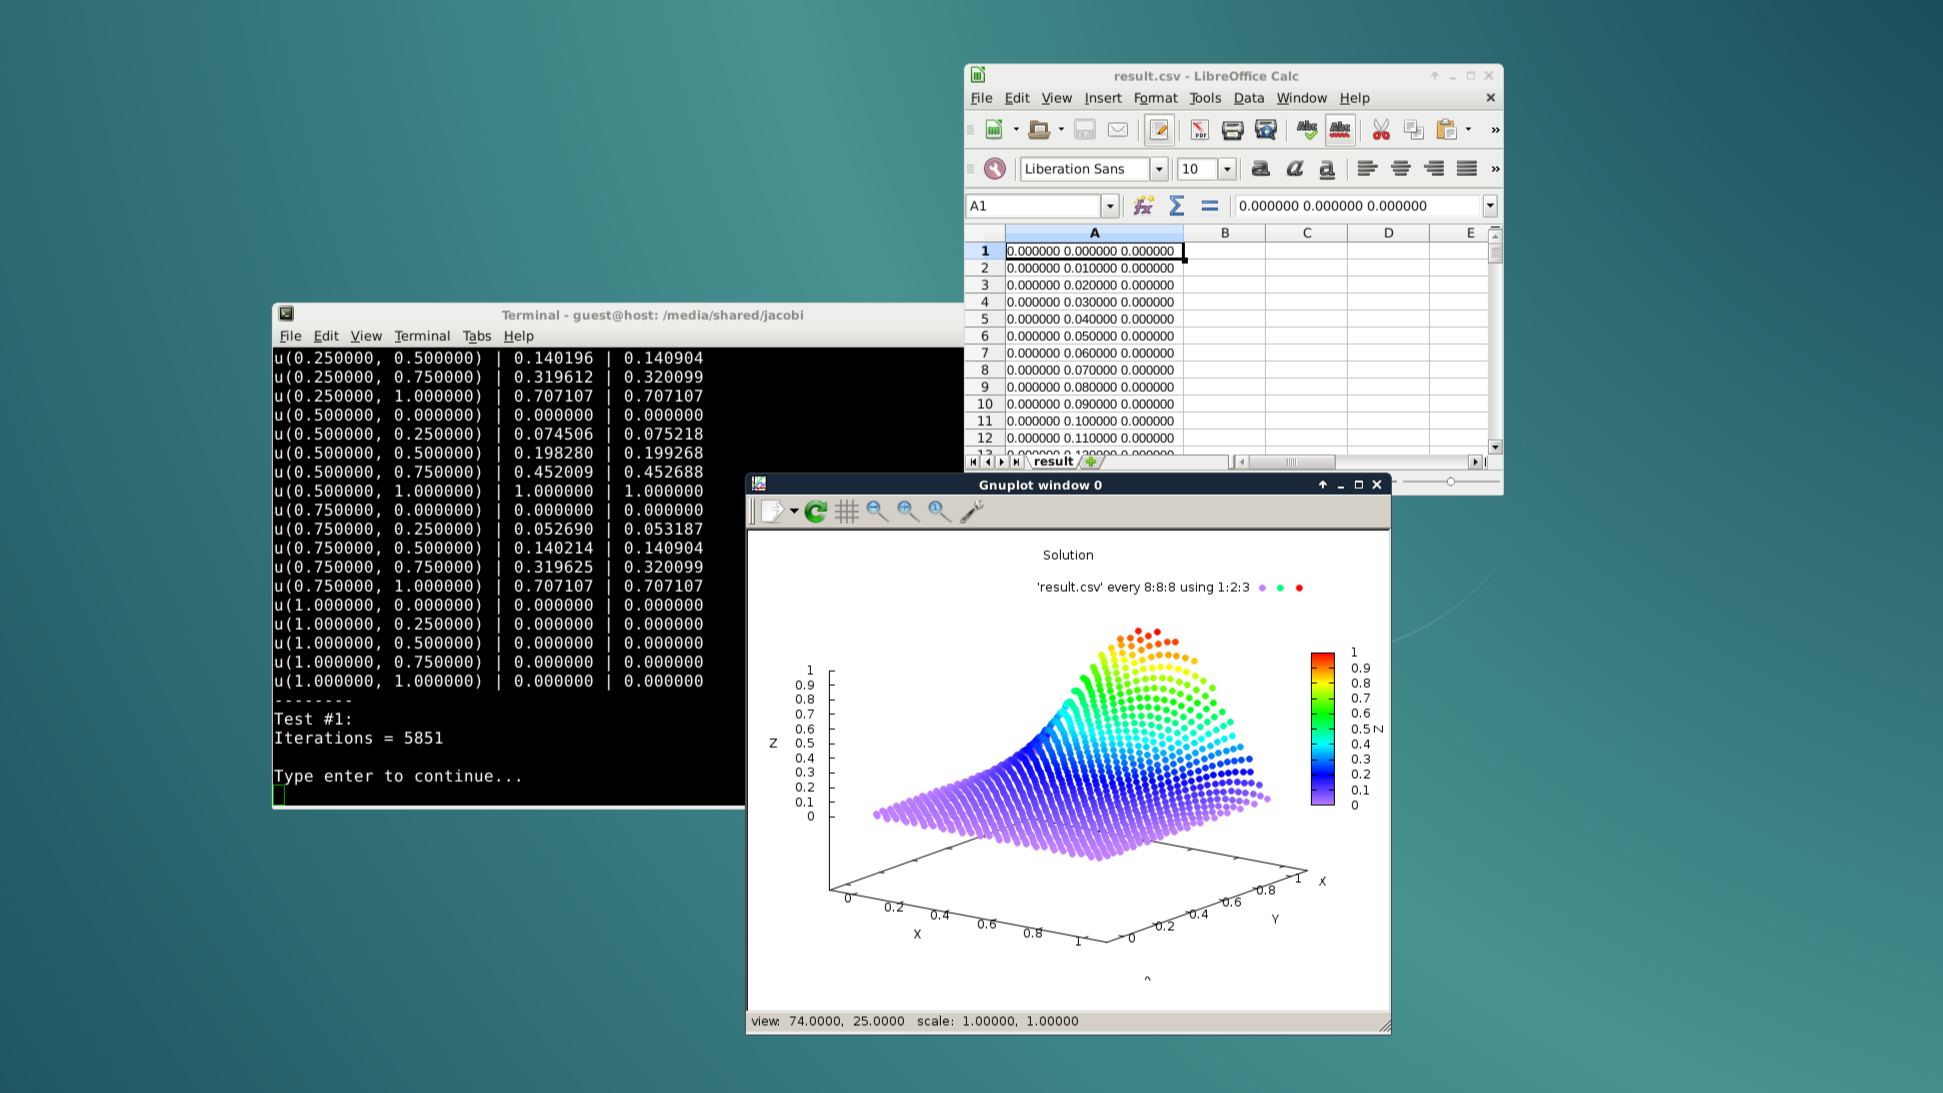
\includegraphics[width=1\textwidth]{preview.png}
\end{figure*}

\begin{thebibliography}{2}
\renewcommand{\bibname}{Литература}
\bibitem{kostomarov}
Костомаров Д.\,П., Фаворский А.\,П. \textit{Вводные лекции по численным методам}. — М.: Логос, 2004. — 184 с.
\bibitem{samarskiy}
Самарский А.\,А. \textit{Введение в численные методы}. — М.: Наука, 1989. — 416 с.
\end{thebibliography}

\end{document}
